% !TEX root = ../../main.tex


\begin{figure}[!htb]
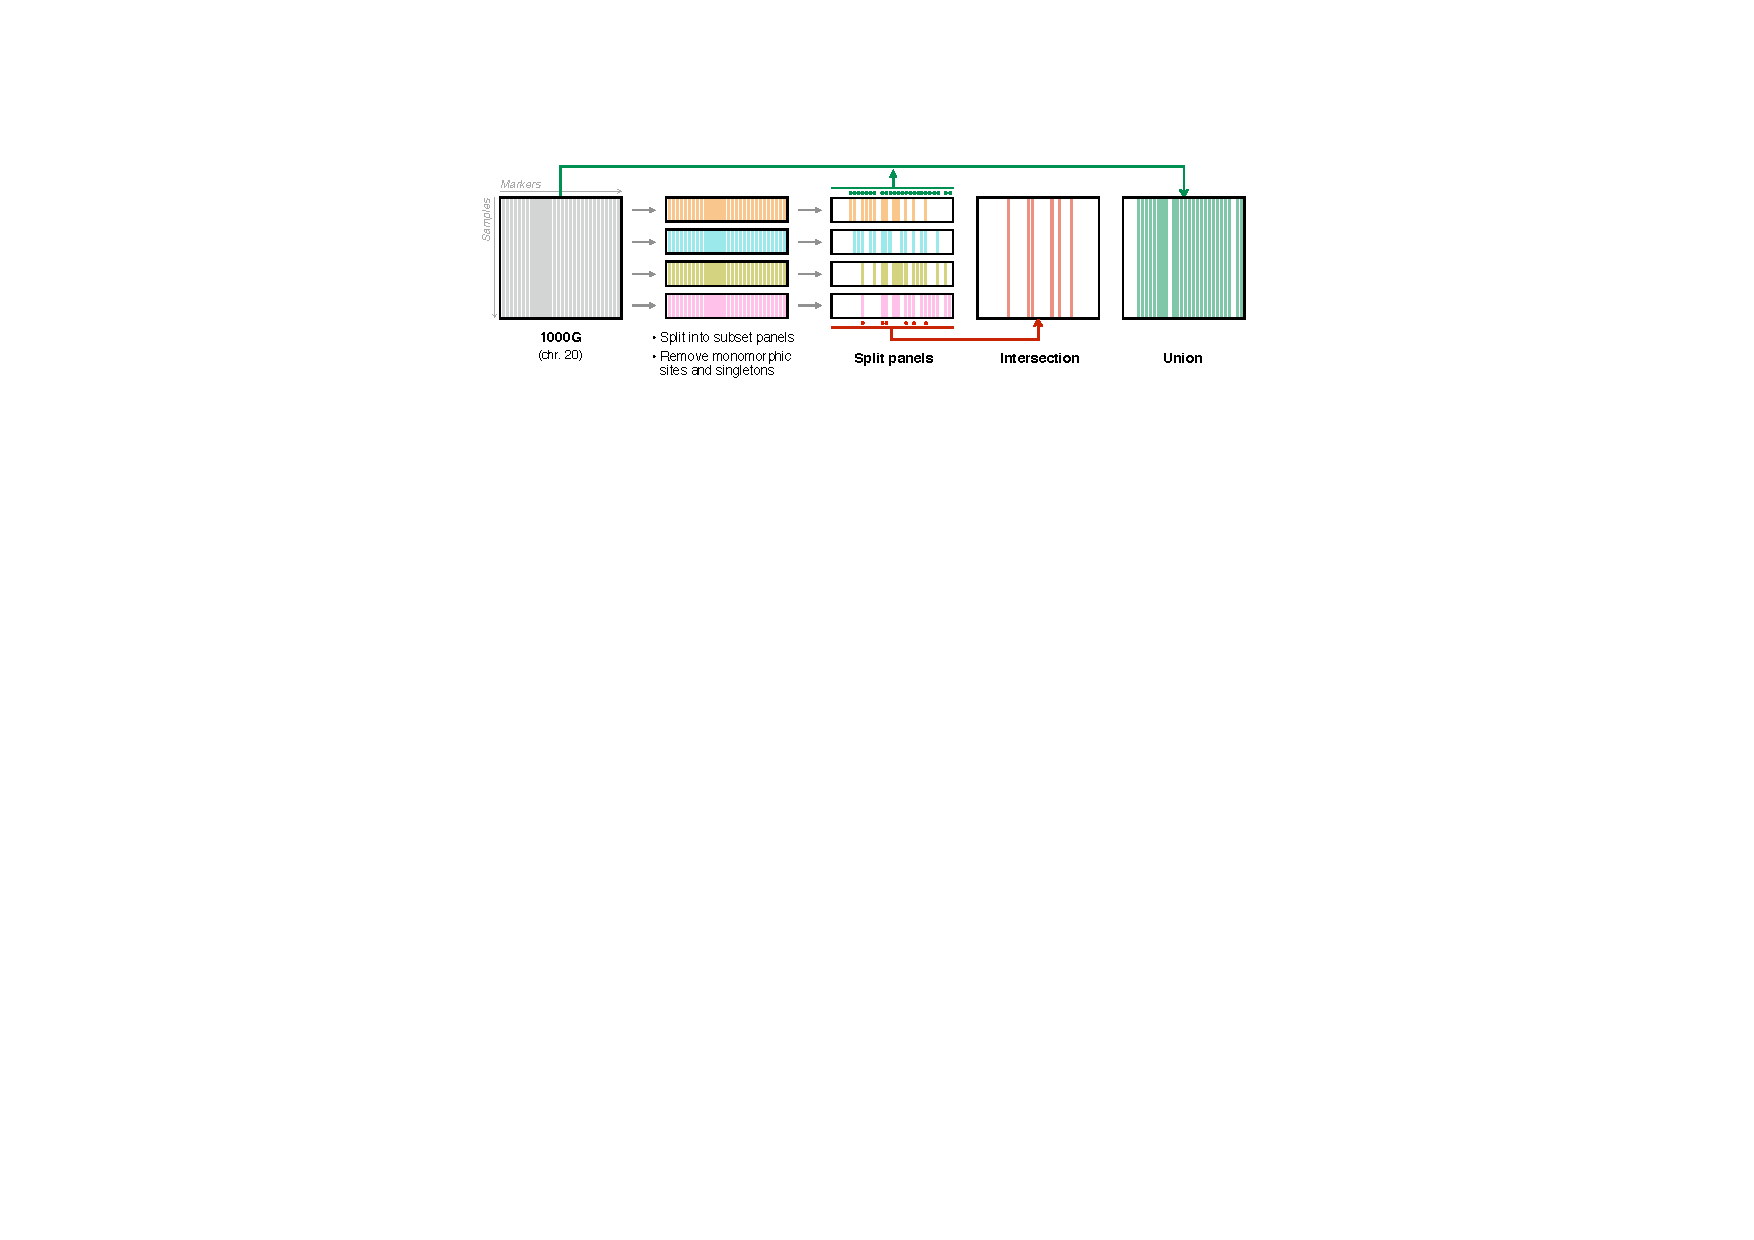
\includegraphics[width=\textwidth]{./img/ch2/info_design_panels}
\Caption{Generation of reference panels in each scenario}
{The original 1000 Genomes dataset (Phase~\rom{1}, chromosome~20) was used to generate multiple, smaller panels for imputation.
This was done in \n{2} scenarios to create data of similar or distinct ethnic backgrounds.
In each scenario, data were split into \n{4} \emph{split} panels of approximately equal size.
Monomorphic sites and singletons were removed in each split panel.
\N{2} additional panels were generated from the obtained split panels per scenario;
\n{1} \emph{intersection} panel and \n{1} \emph{union} panel, both of which contained the union of individuals across split panels, but where the intersection panel only included sites if captured in all split panels, and the union panel included all sites as observed in the original dataset (except monomorphic or singleton sites as per the individuals included).}
{fig:info_design_panels}
\end{figure}
